\documentclass[tikz,border=8pt]{standalone}
% Shared look for every TikZ diagram. Load with \input{../../tools/tikz-style.tex}
\usepackage[T1]{fontenc}
\usepackage{lmodern}
\renewcommand{\sfdefault}{lmr}  % diagrams use the same serif as the text
\usetikzlibrary{arrows.meta, positioning, shapes.geometric, calc, fit, backgrounds}
\definecolor{cblue}{HTML}{4C78A8}
\definecolor{corange}{HTML}{F58518}
\definecolor{cgreen}{HTML}{54A24B}
\definecolor{cred}{HTML}{E45756}
\definecolor{cpurple}{HTML}{B279A2}
\definecolor{cgrey}{HTML}{6B6B6B}
\tikzset{
  every picture/.style={font=\sffamily, line width=1.2pt},
  box/.style={draw=#1, fill=#1!12, rounded corners=4pt, align=center, inner sep=7pt, minimum height=1.1cm},
  box/.default=cgrey,
  arrow/.style={-{Stealth[length=3mm]}, draw=cgrey, line width=1.4pt},
  title/.style={font=\sffamily\bfseries\Large},
  note/.style={font=\sffamily\small, text=cgrey, align=center},
}
\AtBeginDocument{\hyphenpenalty=10000 \exhyphenpenalty=10000}

% LaValle 11.5.1 sensor catalogue, four kinds used in this chapter. Robot at (2, 2, 0) in the 5 m x 4 m room.
\begin{document}
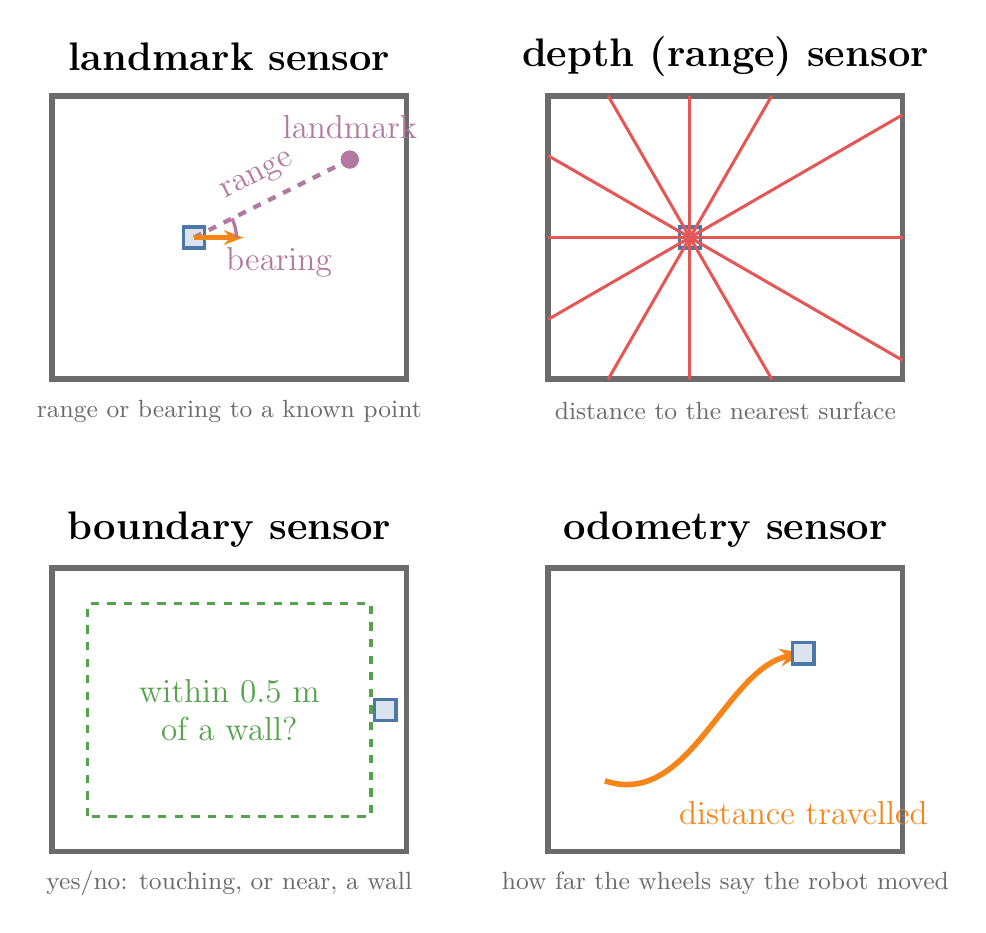
\begin{tikzpicture}[every node/.append style={font=\large}]
  \tikzset{room/.style={draw=cgrey, line width=2pt}, rob/.style={draw=cblue, fill=cblue!20}}
  % panel 1: landmark sensor
  \begin{scope}[shift={(0,0)}, scale=0.9]
    \draw[room] (0,0) rectangle (5,4);
    \draw[rob] (1.85,1.85) rectangle (2.15,2.15);
    \fill[cpurple] (4.2,3.1) circle (0.13); \node[cpurple, above] at (4.2,3.25) {landmark};
    \draw[cpurple, line width=1.6pt, dashed] (2,2) -- (4.2,3.1);
    \draw[corange, -{Stealth[length=2.5mm]}, line width=1.6pt] (2,2) -- (2.7,2);
    \draw[cpurple, line width=1.2pt] (2.6,2) arc (0:26.6:0.6); \node[cpurple] at (3.2,1.65) {bearing};
    \node[cpurple, rotate=27] at (2.9,2.85) {range};
    \node[title] at (2.5,4.55) {landmark sensor};
    \node[note] at (2.5,-0.45) {range or bearing to a known point};
  \end{scope}
  % panel 2: depth (range) sensor
  \begin{scope}[shift={(6.3,0)}, scale=0.9]
    \draw[room] (0,0) rectangle (5,4);
    \draw[rob] (1.85,1.85) rectangle (2.15,2.15);
    \foreach \a/\t in {0/3.000,30/3.464,60/2.309,90/2.000,120/2.309,150/2.309,180/2.000,210/2.309,240/2.309,270/2.000,300/2.309,330/3.464} \draw[cred, line width=1.1pt] (2,2) -- ++(\a:\t);
    \node[title] at (2.5,4.55) {depth (range) sensor};
    \node[note] at (2.5,-0.45) {distance to the nearest surface};
  \end{scope}
  % panel 3: boundary sensor
  \begin{scope}[shift={(0,-6)}, scale=0.9]
    \draw[room] (0,0) rectangle (5,4);
    \draw[cgreen, dashed, line width=1.2pt] (0.5,0.5) rectangle (4.5,3.5);
    \draw[rob] (4.55,1.85) rectangle (4.85,2.15);
    \node[cgreen, align=center] at (2.5,2) {within 0.5 m\\ of a wall?};
    \node[title] at (2.5,4.55) {boundary sensor};
    \node[note] at (2.5,-0.45) {yes/no: touching, or near, a wall};
  \end{scope}
  % panel 4: odometry sensor
  \begin{scope}[shift={(6.3,-6)}, scale=0.9]
    \draw[room] (0,0) rectangle (5,4);
    \draw[corange, line width=2pt, -{Stealth[length=3mm]}] (0.8,1) .. controls (2,0.6) and (2.5,2.6) .. (3.6,2.8);
    \draw[rob] (3.45,2.65) rectangle (3.75,2.95);
    \node[corange] at (3.6,0.55) {distance travelled};
    \node[title] at (2.5,4.55) {odometry sensor};
    \node[note] at (2.5,-0.45) {how far the wheels say the robot moved};
  \end{scope}
\end{tikzpicture}
\end{document}
